\newpage
\section{Containers} \label{container}
\subsection{Differenze tra VM e Container}
Sia nelle macchine virtuali e Container vi è un livello di \textbf{virtualizzazione} (hypervisor e docker engine) ma nei Container manca il sistema operativo guest e il container manager sostituisce l'hypervisor. Inoltre i Container hanno altri vantaggi:
\begin{itemize}
    \item Sono più leggeri, ovvero un Container chiede ad un server meno risorse rispetto ad una macchina virtuale
    \item I tempi di avvio sono molto più brevi rispetto ad una macchina virtuale
    \item Sono più semplici da costruire rispetto ad una macchina virtuale
\end{itemize}
Tuttavia, i Container condividono più risorse all’interno di un server fisico e questo implica che c’è meno isolamento rispetto ad una macchina virtuale, e quindi c’è una superficie più ampia per attacchi di sicurezza. In altre parole un Container è meno sicuro rispetto ad una macchina virtuale.
\begin{figure}[h!]
    \centering
    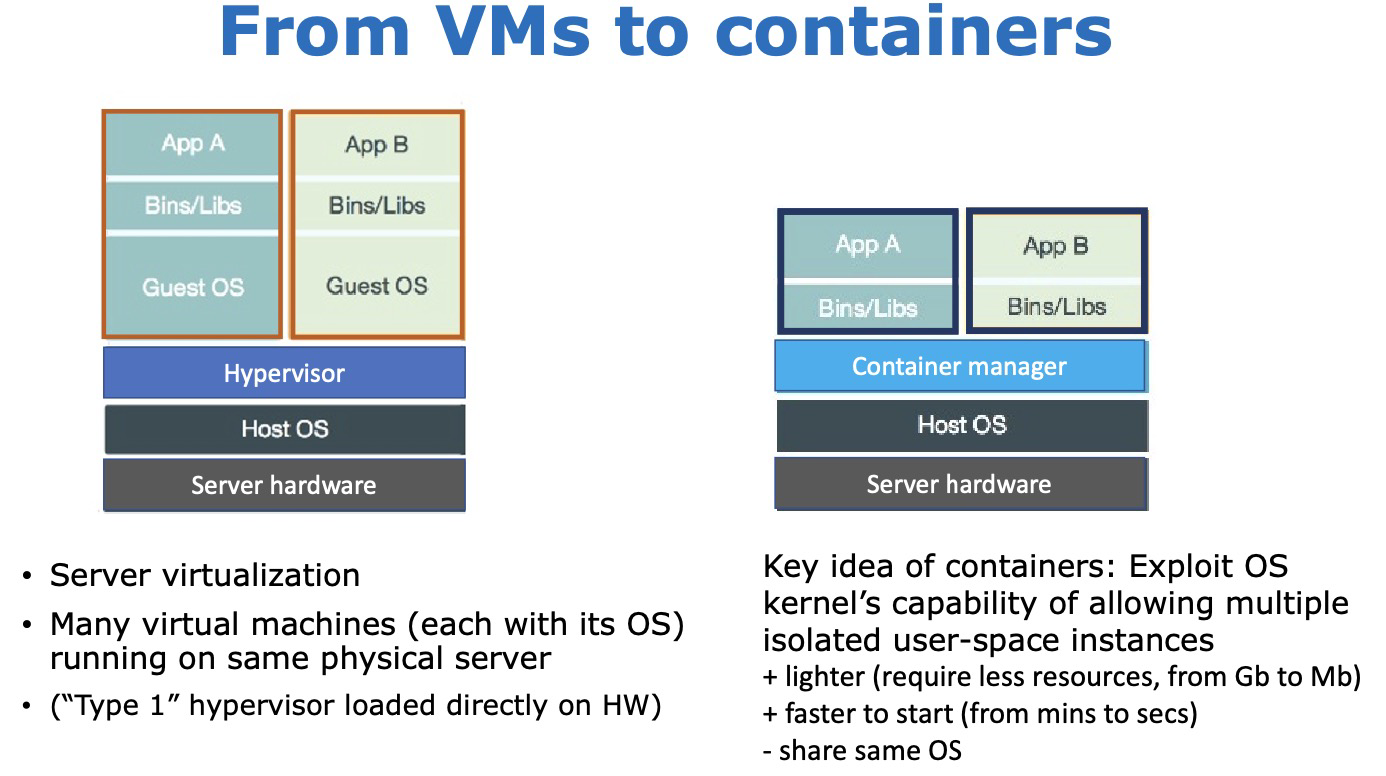
\includegraphics[width=0.5\textwidth]{7.png}
    \caption{VM e Container}
    \label{fig:enter-label}
\end{figure}

\subsection{Docker}
\paragraph{Storia di Docker} I container non sono un'idea molto recente, infatti il sistema operativo UNIX forniva un comando \verb|chroot| che permetteva una forma di isolamento del filesystem.\\
La prima soluzione completa basata su Container fu LXC di Linux Container nel 2008. Nel 2013 il fenomeno è ”esploso” con Docker, che ha aggiunto la portabilità delle immagini e un'interfaccia user-friendly.\\
Docker offre un \textbf{docker engine} per la creazione ed esecuzione di Container e \textbf{docker hub} per pubblicare e scaricare immagini di Container

\paragraph{Come funziona} Docker è una piattaforma che consente di eseguire applicazioni in ambiente isolato, dando la possibilità di sviluppare ed eseguire applicazioni \textbf{portabili} grazie ai containers.\\
In pratica, Docker sfrutta la virtualizzazione basata sui container per eseguire più istanze isolate sullo stesso sistema operativo.
I Container sono \textbf{volatili} ovvero non tengono traccia dei dati una volta terminata l’esecuzione. Per garantire che i dati siano persistenti esistono  i \textbf{volumi}.\\
L’applicazione viene impacchettata in una \textbf{immagine} ovvero un file read-only che rappresenta l’intera applicazione e che permette di mandare in esecuzione un Container. I template (immagini) vengono memorizzati in un \textbf{registry} (per esempio Docker registry) che è strutturato in repositories. Ogni repository contiene un insieme di immagini per versioni diverse del software.\\
Le immagini vengono identificate dalle coppie \textit{repository:tag} e sono \textbf{stratificabili}, cioè strutturate in livelli (layers): al livello più basso vi è il \textit{base image}.\\
Il Container andrà in esecuzione in cima a questa pila di layers e a seconda del tipo di applicazione può effettuare delle modifiche che possono a loro volta essere committate in una nuova immagine.\\

\newpage
\paragraph{Commands} I comandi principali da conoscere per Docker sono:
\begin{itemize}
    \item \verb|pull| scarica un’immagine da un Docker registry
    \item \verb|run| manda in esecuzione il Container definito dall’immagine
    \item \verb|commit| per creare ed effettuare delle modifiche, committate in una nuova immagine
    \item \verb|build| per costruire l'immagine partendo da un \textbf{Dockerfile}, che funziona come una sorta di Makefile
\end{itemize}

\begin{figure}[h!]
    \centering
    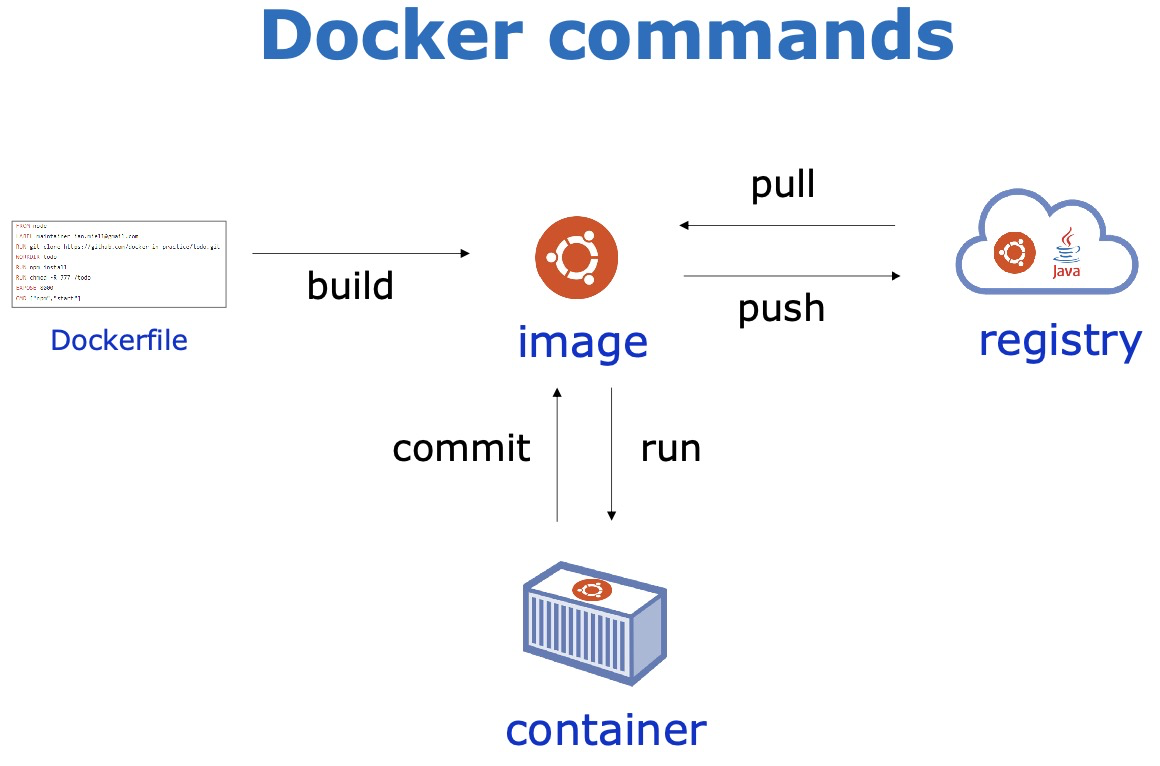
\includegraphics[width=0.7\textwidth]{8.png}
    \caption{Comandi principali di Docker}
    \label{fig:enter-label}
\end{figure}

\paragraph{Demo (DIY)} In \href{https://www.youtube.com/watch?v=YFl2mCHdv24}{questa demo} viene usato un volume per aggiornare la pagina web real time (come già detto, con i volumi i dati sono persistenti)
Il \verb|docker-compose| permette di specificare come si vuole che sia formata l’applicazione multiservizio da mandare in esecuzione.\\
\href{https://www.youtube.com/watch?v=Qw9zlE3t8Ko}{Docker Compose video visto in aula}

\begin{figure}[h!]
    \centering
    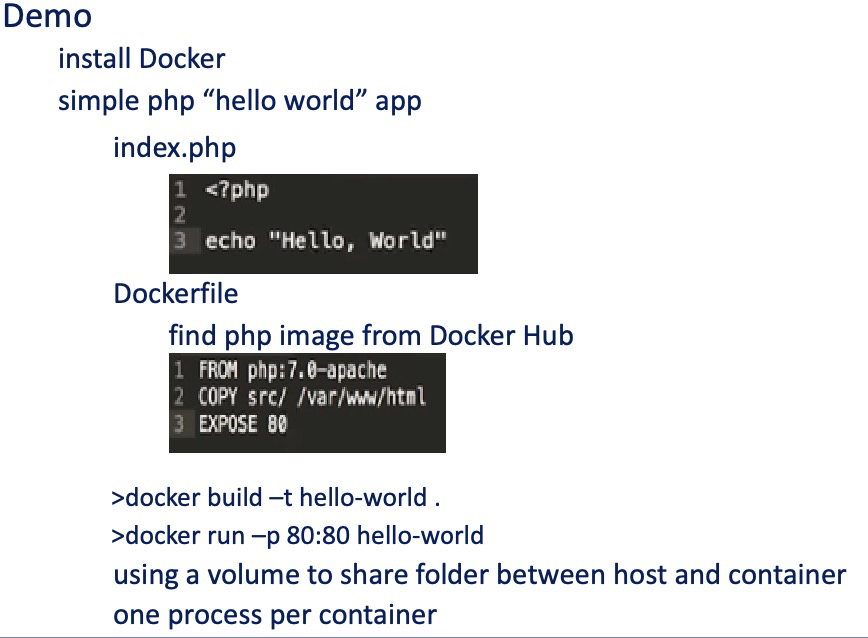
\includegraphics[width=0.5\textwidth]{9.png}
    \caption{Docker demo}
    %\label{fig:enter-label}
\end{figure}

\paragraph{Docker Swarm} Un’altra feature di Docker è la \textbf{swarm mode}, un approccio dichiarativo (l'utente dichiara l'organizzazione che desidera ottenere) che permette di gestire un insieme (cluster) di host Docker chiamati \textit{swarm}.\\
Quindi i vari task vengono ripartiti tra host diversi. I nodi del cluster possono avere due ruoli:
\begin{itemize}
    \item \textit{manager}, che delegano e distribuiscono i task ai workers
    \item \textit{workers}, che eseguono i task
\end{itemize}
L’utente può definire lo stato per la configurazione a tempo di esecuzione dell’applicazione. Gli swarm manager effettuano un \textbf{monitoraggio costante} delle attività e interviene qualora vi sia una differenza tra lo stato attuale e lo stato desiderato dall’utente.\\
Per esempio se l’utente desidera che vi siano in esecuzione 10 repliche dello stesso container, il manager swarm distribuisce le 10 repliche sulle macchine workers; se una worker machine ospita due repliche e si blocca, il manager swarm crea due nuove repliche che vengono assegnate ad altre worker machine disponibili ed in esecuzione
\begin{figure}[h!]
    \centering
    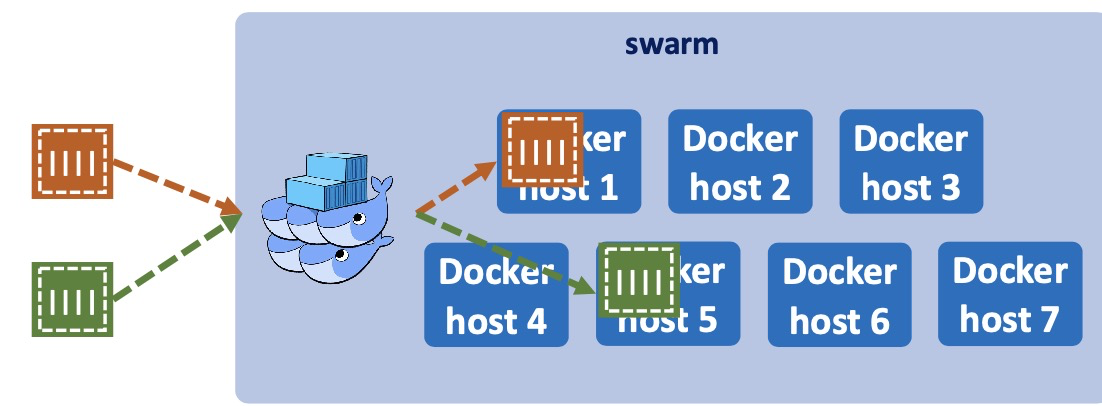
\includegraphics[width=0.7\textwidth]{10.png}
    \caption{Docker swarm}
    %\label{fig:enter-label}
\end{figure}

\subsection{Kubernetes}
Nel 2014, dopo il successo di Docker, è stato lanciato Kubernetes che è un sistema per l'orchestrazione di Container. Kubernetes possiede molte funzionalità simili a Docker swarm ma è più efficiente. Docker e Kubernetes non sono in contrapposizione tra di loro, ma si integrano a vicenda.\\
Un \textbf{pod} è un gruppo di uno o più Containers con storage/rete condivisa, e con una specifica per come gestire i Container. I contenuti del pod vengono allocati e schedulati per essere eseguite in contesto condiviso.\\
Un \textbf{kubelet} è un \textit{node agent} che è in esecuzione \textbf{su ogni nodo} che prende un insieme di specifiche pod (principalmente attraverso il server API) e assicura che i Container descritti in tali specifiche siano in esecuzione e ”sani”.\\
\href{https://www.youtube.com/watch?v=PH-2FfFD2PU}{Video su Kubernetes visto in aula}

\paragraph{Docker Swarm vs Kubernetes} Così come docker swarm, anche kubernetes serve per l'orchestrazione di containers. La differenza sta nella semplicità e nella potenza: Swarm è più semplice da installare ed è abbastanza semplice da imparare. Kubernetes offre il meccanismo di \textbf{auto-scaling}, è più robusto in termini di tolleranza ai guasti.\\
Quindi se l’applicazione che si deve gestire è relativamente semplice, Docker Swarm probabilmente è la scelta giusta. Se invece l’applicazione raggiunge un livello di complessità considerevole e la dimensione dei cluster non è banale, allora è consigliabile usare  Kubernetes.